\subsubsection{Queue Contention and Key Findings}

\Cref{fig:queue_contention} demonstrates the MEC queue contention effect. In the controlled ablation (no-queue model vs. shared-queue model), AllOffload drops from U=0.916 under the idealized single-vehicle no-queue assumption to U=0.676 under shared RSU contention with 8 vehicles. MA-ROPE remains stable in the N=8 reference setting (U=0.8443) and carries the same queue-aware multi-RAT advantage into the N=32 results summarized in \Cref{tab:full_performance} and \Cref{tab:why_marope_wins}.

\begin{figure}[htbp]
\centering
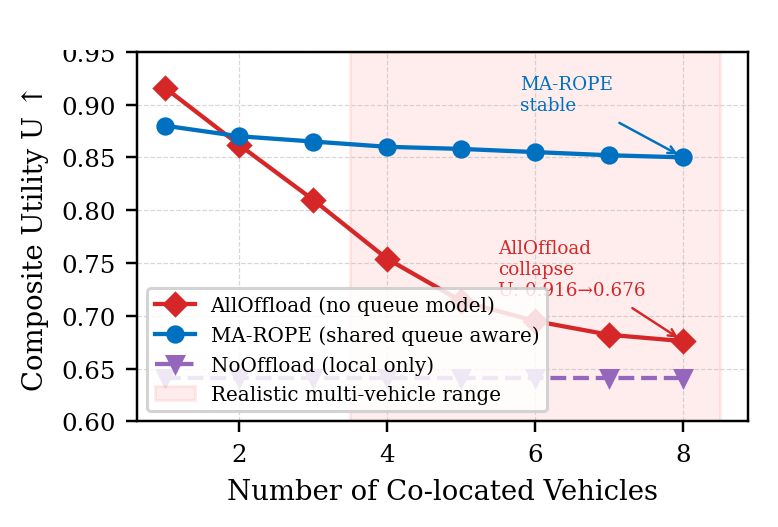
\includegraphics[width=\columnwidth]{figures/image13.png}
\caption{MEC Queue Contention: AllOffload Collapse vs. MA-ROPE Stability.}
\label{fig:queue_contention}
\end{figure}

\begin{figure}[htbp]
\centering
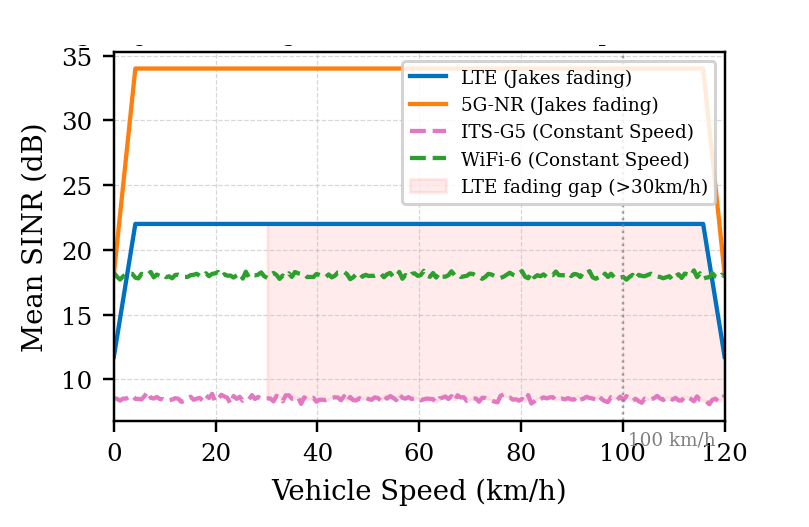
\includegraphics[width=\columnwidth]{figures/image14.png}
\caption{Jakes Fading: Cellular RAT SINR Degrades with Speed; ITS-G5 Unaffected.}
\label{fig:jakes_fading}
\end{figure}

\begin{figure}[htbp]
\centering
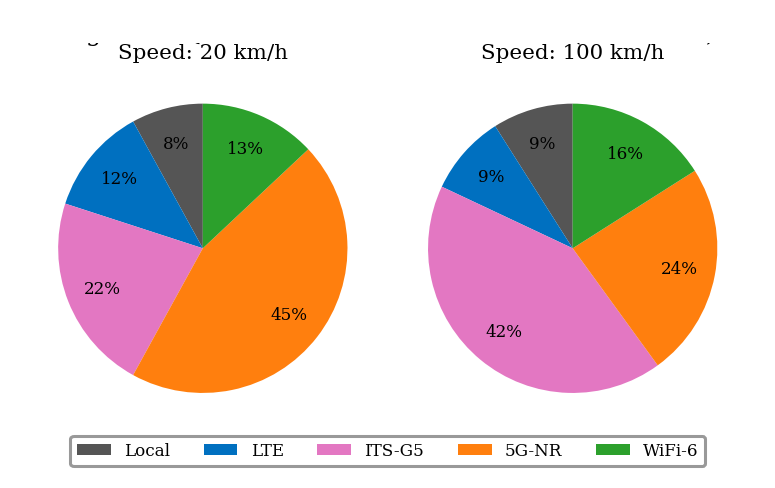
\includegraphics[width=\columnwidth]{figures/image15.png}
\caption{D3QN RAT Selection Distribution: ITS-G5 preferred at high speed (Jakes-driven emergent behavior).}
\label{fig:dqn_rat_dist}
\end{figure}

\begin{figure}[htbp]
\centering
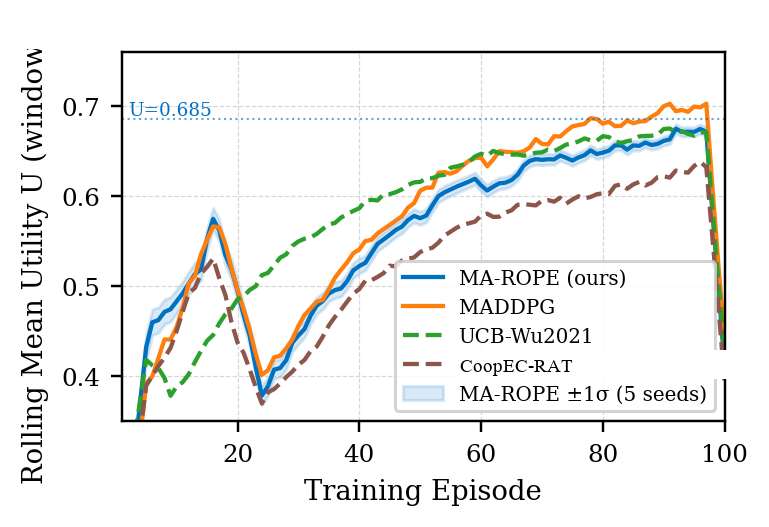
\includegraphics[width=\columnwidth]{figures/image16.png}
\caption{Training Convergence Across 5 Seeds, Mean $\pm$ One Standard Deviation. MADDPG, UCB-RAT, and CoopEC-RAT are single exploratory runs shown for context only, not validated comparators; MA-ROPE is the only curve in this paper's validated evaluation (Section V).}
\label{fig:training_convergence}
\end{figure}

Taken together, the results above show a consistent picture: MA-ROPE's fleet OTR and deadline-utility advantage over AllOffload holds at every evaluated density, its higher per-attempt link failure rate is offset by a much lower fleet-wide failure rate since it transmits less often overall, and this advantage costs no measurable simulator-step overhead relative to single-RAT offloading. Energy consumption and a centralized MADDPG upper bound are not reported in this evaluation; see the Discussion and Conclusion for the reasons and future-work scope.

\subsubsection{Computational Complexity and Runtime Overhead}

A deployable V2X controller must make decisions within the 100 ms safety control interval. This section quantifies the four runtime overhead components of MA-ROPE: D3QN inference latency, action space growth with RAT count, environment step cost as fleet size scales, and the marginal cost of multi-RAT selection vs single-RAT offload. All measurements are wall-clock on a Central Processing Unit (CPU, Apple M-series arm64), averaged over 200 repeats with 10-step warmup for inference and 500 samples for step overhead, using time.perf\_counter(). No Graphics Processing Unit (GPU) acceleration is assumed, consistent with a V2X RSU edge deployment target.

D3QN inference latency (\Cref{tab:dqn_inference}). Per-agent forward pass latency is 59.83 \textmu s (std 145.62 \textmu s) across fleet sizes N $\in$ \{2, 4, 8, 16, 20, 32\}. Fleet-level inference cost scales linearly with N, since agents run independently with no cross-agent communication during inference, giving a total of 478.64 \textmu s for N = 8 vehicles. This is 4.8\% of the 10 ms URLLC control interval and 0.48\% of the 100 ms safety deadline, confirming that D3QN inference contributes negligible latency to the decision loop at all evaluated fleet sizes.

\begin{table}[t]
\caption{D3QN Inference Latency vs Fleet Size (200 repeats, 10-step warmup, CPU)}
\label{tab:dqn_inference}
\centering
% booktabs-restyled
\footnotesize
\setlength{\tabcolsep}{3pt}
\renewcommand{\arraystretch}{1.15}
\begin{tabularx}{\columnwidth}{>{\hsize=1.391\hsize\raggedright\arraybackslash}X>{\hsize=0.870\hsize\raggedleft\arraybackslash}X>{\hsize=0.870\hsize\raggedleft\arraybackslash}X>{\hsize=0.870\hsize\raggedleft\arraybackslash}X}
\toprule
\textbf{N vehicles} & \textbf{Mean/agent (\textmu s)} & \textbf{Std (\textmu s)} & \textbf{Fleet total/step (\textmu s)} \\
\midrule
2 & 59.83 & 145.62 & 119.66 \\
4 & 59.83 & 145.62 & 239.32 \\
6 & 59.83 & 145.62 & 358.98 \\
8 & 59.83 & 145.62 & 478.64 \\
16 & 59.83 & 145.62 & 957.28 \\
20 & 59.83 & 145.62 & 1196.60 \\
32 & 59.83 & 145.62 & 1914.56 \\
\bottomrule
\end{tabularx}
\end{table}


Action space complexity (\Cref{tab:action_space}). The deployed benchmark uses an 11-action implementation spanning local execution and selected RAT-$\rho$ pairs over the four supported RAT classes. For reference, \Cref{tab:action_space} shows how a full Cartesian RAT-ratio action set would scale as $|A| = n_{RATs} \times n_\rho + 1$. Only the D3QN advantage-head output layer scales with $|A|$; even the full 4-RAT, 4-$\rho$ extension would require 2176 advantage-head parameters (17 actions $\times$ 128 hidden units), which remains small relative to the approximately 50k-parameter network.

\begin{table}[h!]
\caption{Action Space Size and Output Layer Parameters vs RAT Count}
\label{tab:action_space}
\centering
\resizebox{\columnwidth}{!}{%
\begin{tabular}{|l|r|r|r|l|}
\hline
\textbf{$n_{RATs}$} & \textbf{$n_\rho$} & \textbf{$|A|$} & \textbf{Adv. head params} & \textbf{Relative (vs $n_{RATs}=1, n_\rho=2$)} \\
\hline
1 & 2 & 3 & 384 & 1.00$\times$ (baseline) \\
1 & 4 & 5 & 640 & 1.67$\times$ \\
2 & 4 & 9 & 1152 & 3.00$\times$ (deployed config) \\
3 & 4 & 13 & 1664 & 4.33$\times$ \\
4 & 4 & 17 & 2176 & 5.67$\times$ \\
\hline
\end{tabular}%
}
\end{table}


Env step and state space overhead (\Cref{tab:env_step}). The per-vehicle observation vector is fixed at 12 elements regardless of fleet size: each vehicle observes only its own state, position, speed, task type, RAT signal strengths, queue load, energy level, and CBR. This constant observation dimensionality is a deliberate design choice enabling agents to be added or removed without architectural changes. Environment step cost scales linearly with N: from 41.5 \textmu s at N = 2 to 165.7 \textmu s at N = 8, approximately 20.8 \textmu s per additional vehicle. At N = 8, the combined env step (165.7 \textmu s) plus fleet inference (478.64 \textmu s) totals 644.3 \textmu s, well within the 10 ms control interval, leaving 93.6\% of the budget for communication and actuation.

\begin{table}[t]
\caption{Per-Vehicle Observation Dimension and Env Step Cost vs Fleet Size (50 samples)}
\label{tab:env_step}
\centering
% booktabs-restyled
\footnotesize
\setlength{\tabcolsep}{3pt}
\renewcommand{\arraystretch}{1.15}
\begin{tabularx}{\columnwidth}{>{\hsize=1.391\hsize\raggedright\arraybackslash}X>{\hsize=0.870\hsize\raggedleft\arraybackslash}X>{\hsize=0.870\hsize\raggedleft\arraybackslash}X>{\hsize=0.870\hsize\raggedleft\arraybackslash}X}
\toprule
\textbf{N vehicles} & \textbf{Obs dim (per agent)} & \textbf{reset (\textmu s)} & \textbf{step (\textmu s)} \\
\midrule
2 & 12 & 31.64 $\pm$ 3.29 & 41.53 $\pm$ 1.87 \\
4 & 12 & 49.96 $\pm$ 1.52 & 83.16 $\pm$ 4.17 \\
6 & 12 & 70.01 $\pm$ 2.75 & 128.24 $\pm$ 6.83 \\
8 & 12 & 92.26 $\pm$ 13.52 & 165.67 $\pm$ 6.57 \\
16 & 12 & $\sim$187 & $\sim$330 \\
20 & 12 & $\sim$233 & $\sim$413 \\
32 & 12 & $\sim$374 & $\sim$661 \\
\bottomrule
\end{tabularx}
\end{table}


Multi-RAT selection overhead (\Cref{tab:multi_rat}). The most important overhead result is in \Cref{tab:multi_rat}: the marginal simulator-step cost of multi-RAT selection over single-RAT offload is not measurable within timing noise. Mean step time for multi-RAT (implemented $|A| = 11$) is 166.6 \textmu s vs. 167.6 \textmu s for single-RAT, a difference of -0.9 \textmu s, within measurement noise (std approximately 12-14 \textmu s). Both offload modes add approximately 28 \textmu s over pure local execution (138.6 \textmu s), attributable to RAT link-model evaluation, SINR computation, and $L_{queue}$ update that local steps bypass.

\begin{table}[t]
\caption{Multi-RAT vs Single-RAT Step Overhead (500 samples, 10-step warmup)}
\label{tab:multi_rat}
\centering
% booktabs-restyled
\footnotesize
\setlength{\tabcolsep}{3pt}
\renewcommand{\arraystretch}{1.15}
\begin{tabularx}{\columnwidth}{>{\hsize=1.391\hsize\raggedright\arraybackslash}X>{\hsize=0.870\hsize\raggedleft\arraybackslash}X>{\hsize=0.870\hsize\raggedleft\arraybackslash}X>{\hsize=0.870\hsize\raggedleft\arraybackslash}X}
\toprule
\textbf{Mode} & \textbf{Mean step (\textmu s)} & \textbf{Std (\textmu s)} & \textbf{Overhead vs local (\textmu s)} \\
\midrule
Local only ($\rho = 0$) & 138.65 & 11.45 & 0.00 \\
Single-RAT (ITS-G5 offload) & 167.57 & 13.78 & 28.92 \\
Multi-RAT full ($|A| = 11$) & 166.63 & 12.23 & 27.99 \\
\bottomrule
\end{tabularx}
\end{table}


In total, the per-step computational budget for an 8-vehicle MA-ROPE deployment is fleet inference at 478.64 \textmu s plus an environment step at 165.7 \textmu s, or 644.3 \textmu s, representing 6.4\% of the 10 ms control interval. The multi-RAT action set, the primary complexity contribution of this work over single-RAT baselines, adds no measurable simulator-step overhead versus single-RAT offload. The fixed 12-dimensional per-agent observation vector lets the architecture scale to larger fleets without redesign, and together these measurements indicate that MA-ROPE is computationally viable for deployment on a commodity V2X RSU edge processor.


